\documentclass[UTF8,a4paper,zihao=-4]{ctexart}

\usepackage[left=2.45cm,right=2.45cm,top=2.45cm,bottom=2.35cm]{geometry}
\usepackage{amsmath,amssymb}
\usepackage{graphicx}
\usepackage{booktabs}
\usepackage{tabularx}
\usepackage{array}
\usepackage{longtable}
\usepackage{enumitem}
\usepackage{caption}
\usepackage{float}
\usepackage{fancyhdr}
\usepackage{xcolor}
\usepackage{tikz}
\usepackage{hyperref}
\usetikzlibrary{arrows.meta,positioning,fit,shapes.geometric}

\graphicspath{{figures/}}
\definecolor{zjublue}{HTML}{145DA0}
\definecolor{softblue}{HTML}{EAF2F8}
\definecolor{softgreen}{HTML}{EAF4EA}
\definecolor{softorange}{HTML}{FFF2DF}
\definecolor{softgray}{HTML}{F3F4F5}
\hypersetup{colorlinks=true,linkcolor=zjublue,urlcolor=zjublue}
\setlength{\parindent}{2em}
\setlength{\parskip}{0.15em}
\setlength{\headheight}{15pt}
\setlength{\emergencystretch}{2em}
\linespread{1.35}
\setlist[itemize]{leftmargin=2em,itemsep=0.2em,topsep=0.25em}
\setlist[enumerate]{leftmargin=2.4em,itemsep=0.2em,topsep=0.25em}
\captionsetup{font=small,labelsep=quad}
\renewcommand{\arraystretch}{1.25}
\newcolumntype{Y}{>{\centering\arraybackslash}X}
\newcolumntype{L}[1]{>{\raggedright\arraybackslash}p{#1}}

\ctexset{
  section={format=\bfseries\zihao{3},beforeskip=1.4em,afterskip=0.7em},
  subsection={format=\bfseries\zihao{4},beforeskip=1em,afterskip=0.45em},
  subsubsection={format=\bfseries\zihao{-4},beforeskip=0.7em,afterskip=0.3em}
}

\pagestyle{fancy}
\fancyhf{}
\fancyhead[L]{面向 CODESYS 的 ST 代码生成 Agent}
\fancyhead[R]{生成式人工智能课程大作业}
\fancyfoot[C]{\thepage}
\renewcommand{\headrulewidth}{0.4pt}

\tikzset{
  box/.style={draw=zjublue,rounded corners=2pt,fill=softblue,minimum height=1.05cm,
    align=center,text width=2.5cm,inner sep=5pt},
  greenbox/.style={box,draw=green!50!black,fill=softgreen},
  orangebox/.style={box,draw=orange!70!black,fill=softorange},
  graybox/.style={box,draw=gray!70,fill=softgray},
  flow/.style={-{Latex[length=2.4mm]},thick,zjublue}
}

\newcommand{\placeholder}{\textcolor{red!75!black}{待补充}}
\newcommand{\linefield}[2]{\underline{\makebox[#1][c]{#2}}}

\begin{document}

\begin{titlepage}
  \centering
  \vspace*{1.0cm}
  
\includegraphics[width=0.68\textwidth]{cover.png}\par
  \vspace{0.7cm}
  
\includegraphics[width=0.15\textwidth]{logo.png}\par
  \vspace{0.8cm}
  {\zihao{2}\bfseries Genai赋能工业编程\par}
  \vspace{1.2cm}
  {\zihao{1}\bfseries 面向 CODESYS 的 ST 代码生成 Agent\par}
  \vspace{0.4cm}
  {\zihao{3}设计、实现与实验评估\par}
  \vspace{1.5cm}
  \renewcommand{\arraystretch}{1.55}
  \begin{tabular}{>{\raggedleft\arraybackslash}p{3.6cm}p{8.0cm}}
    课程名称： & \linefield{7.2cm}{Genai赋能工业编程}\\
    学院专业： & \linefield{7.2cm}{控制科学与工程学院}\\
    小组成员： & \linefield{7.2cm}{\placeholder（五位成员姓名与学号）}\\
    指导教师： & \linefield{7.2cm}{\placeholder}\\
    完成日期： & \linefield{7.2cm}{2026 年 11 月}\\
  \end{tabular}
  \vfill
\end{titlepage}

\pagenumbering{Roman}
\section*{成员分工}
\addcontentsline{toc}{section}{成员分工}
\begin{table}[H]
  \centering
  \begin{tabularx}{\textwidth}{L{2.3cm}L{2.8cm}X}
    \toprule
    姓名 & 学号 & 主要工作\\
    \midrule
    \placeholder & \placeholder & 数据集整理与题目审核\\
    \placeholder & \placeholder & LTL Spec 与测试用例\\
    \placeholder & \placeholder & 自研 harness 与 CODESYS 接入\\
    \placeholder & \placeholder & 基线实验与结果分析\\
    \placeholder & \placeholder & 报告、PPT 与演示整理\\
    \bottomrule
  \end{tabularx}
\end{table}

\section*{摘\quad 要}
\addcontentsline{toc}{section}{摘要}
PLC Structured Text（ST）代码既要满足语言和工程接口要求，也要在扫描周期中实现正确的控制行为。围绕这一问题，本项目整理了由 20 道公共题和 10 道自建题构成的数据集，逐题编写工具无关的 LTL 规约和共享测试用例，共形成 30 道任务、136 条 LTL 性质、92 个测试用例和 352 个测试步骤。在此基础上，我们实现了一个轻量级 Agent harness，完成任务读取、提示词构建、结构化候选解析、接口预检、CODESYS 编译、编译错误反馈、有限轮修复、Simulation 自动测试和证据保存；同时选择 Codex CLI 作为现成 Agent 基线。实验采用两个框架与两个基座模型组成四种设置，在冻结题目、Spec、模型参数、候选次数和测试标准后完成 120 次正式运行。最终有 90 次首次编译通过、96 次在修复范围内通过编译，205/368 个计划测试通过，53 次运行通过本题全部测试，对应最终编译率 80.00\%、测试通过率 55.71\% 和任务成功率 44.17\%。结果显示，可编译代码与功能正确代码之间仍有明显差距；模型差异大于本实验中的框架差异。项目最终形成了一条从自然语言需求到 ST 候选、CODESYS 执行和可追溯评价的完整流程。

\noindent\textbf{关键词：}PLC；Structured Text；Coding Agent；CODESYS；LTL；自动测试

\tableofcontents
\clearpage
\pagenumbering{arabic}

\section{大作业准备}

\subsection{项目思考与讨论}
根据学习，ST 是 IEC 61131-3 标准中的文本化 PLC 编程语言，适合表达状态保持、互锁、顺序控制、定时和数据处理等逻辑。大模型已经能够根据自然语言生成形式完整的程序。但课堂中也提到了PLC 任务与普通算法题存在明显差异：程序会被周期性扫描，输出常常依赖此前状态，停止、急停和故障还具有明确优先级。模型给出代码之后，仍需要真实工程环境确认接口、类型和调用链，再通过功能测试检查控制行为。

课程中关于软件测试的部分指出，如果测试只覆盖少数样例，即使全部通过，程序仍可能在未覆盖输入上出错。基于这个结论，我们适当地调整了本项目的评价方法。所以，我们将问题分成了三个层次，候选结构是否符合题目接口，代码能否通过 CODESYS 编译，运行行为能否通过需求对应的测试。这些也分别对应着后文的报告编译率、测试通过率和任务成功率等

\subsection{项目目标与主要工作}
课程作业要求是在全部公共题和不少于 10 道自建题上，对自研框架、现成 Agent 和两个基座模型进行四种设置比较。围绕这一目标，我们完成了项目的工作流程如下：
\begin{enumerate}
  \item 将公共题和自建题统一为可执行的数据结构（比如json，初期我们也有采用md但是不是很方便读取），并写下自建题的来源、改编、审核和 PLC 合理性；
  \item 完善数据部分之后，我们便逐题编写LTL Spec与测试用例，使自然语言需求可以追踪到具体性质和测试步骤；
  \item 之后开始完善代码部分，打通模型、Python、CODESYS编译与Simulation自动测试，建立生成、检查、修复等的闭环，构建出一个agent harness；
  \item 确保实验条件一致后完成 120 次正式运行，然后从模型、框架、难度和题库类型等角度分析结果。
\end{enumerate}

\begin{figure}[H]
  \centering
  \begin{tikzpicture}[node distance=8mm and 7mm,scale=0.93,transform shape]
    \node[box] (task) {30 道 PLC 任务\\自然语言需求与接口};
    \node[greenbox,right=of task] (spec) {136 条 LTL\\92 个共享测试};
    \node[box,right=of spec] (agent) {自研 harness\\或 Codex CLI};
    \node[orangebox,right=of agent] (model) {DeepSeek\\或 Qwen};
    \node[greenbox,below=of agent] (codesys) {CODESYS\\编译与 Simulation};
    \node[graybox,left=of codesys] (evidence) {响应、候选、错误\\步骤输出与状态};
    \draw[flow] (task) -- (spec);
    \draw[flow] (spec) -- (agent);
    \draw[flow] (agent) -- (model);
    \draw[flow] (model.south) |- (codesys.east);
    \draw[flow] (codesys) -- (evidence);
    \draw[flow] (codesys.north) -- node[right,font=\small]{编译反馈} (agent.south);
  \end{tikzpicture}
  \caption{从需求到结果的关系}
  \label{fig:overview}
\end{figure}

上面是我们的项目主线，首先题目与Spec定义输入和约束，然后Agent与模型产生候选，再之后CODESYS 提供真实编译和测试结果，为了对比公平性呢，我们的所有中间产物会进入一个原始证据目录。报告中的数字由这些记录重新汇总生成，可以更加方便对比和查看。

\section{数据规范}

\subsection{数据集构成}
项目数据集包含老师提供的 20 道公共题和 10 道自建题。公共题采用课程提供；自建题基于ai和我们的检索补充了安全锁存、报警复位、批次流程、定时监控和现场联锁等。最终规模见表~\ref{tab:dataset}。

\begin{table}[H]
  \centering
  \caption{数据集规模}
  \label{tab:dataset}
  \begin{tabular}{lrrrr}
    \toprule
    类型 & 题目数 & LTL 性质 & 测试用例 & 测试步骤\\
    \midrule
    公共题 & 20 & 92 & 62 & 263\\
    自建题 & 10 & 44 & 30 & 89\\
    \midrule
    合计 & 30 & 136 & 92 & 352\\
    \bottomrule
  \end{tabular}
\end{table}

30 道题按统一标准分为 easy 9 道、medium 12 道和 hard 9 道。


\subsection{公共题目转换}
保持原始材料不变，但是实验使用转换后的JSON，这样可以每道题明确任务ID、需求、POU名称与类型、公开接口，以及难度和必要的编译上下文，转换之后可以解决原始题面与自动实验之间的接口衔接。

其中，使用 DUT、数组和 \texttt{VAR\_IN\_OUT} 的题目需要在临时工程中创建固定类型并绑定实例；在分析ai的建议后，我们选择\texttt{public\_18} 的 FIFO 容量统一为 10，元素类型统一为 DINT。

\subsection{自建题流程}
10 道自建题由自主构思 2 道、经验改编 6 道和规则合成 2 道组成，难度分布为 easy 3 道、medium 4 道、hard 3 道。

题目构建结合老师提供的公共题，遵循相同过程。先从现场控制场景提取一个边界清晰的功能任务，再确定公开输入输出和初始状态，补充急停、故障、复位、保持或最小时间等规则，最后由题面、Spec和测试交叉审核。

例如，在题目生成后，我们进行微调，在\texttt{custom\_01}中强调急停锁存与人工复位，\texttt{custom\_06} 包含填充、混合、排空的批次状态推进，\texttt{custom\_09} 关注输送机在时间窗口内的堵料监测。这些任务能够用 PLC 扫描周期和现场信号自然表达，也覆盖了从布尔控制到多阶段时序逻辑的变化。由于我们的自编题接口、定义可能更加规范，所以后面在实验的时候自编的数据会表现得更好。

\begin{table}[H]
  \centering
  \caption{选取部分自编题说明}
  \begin{tabularx}{\textwidth}{L{2.3cm}L{2.5cm}L{2.0cm}X}
    \toprule
    题目 & 场景 & 考虑难点 & 人工审核修改点\\
    \midrule
    \texttt{custom\_01} & 设备安全锁存 & 安全优先级 & 急停解除后不得自动恢复，必须人工复位\\
    \texttt{custom\_06} & 配料批次流程 & 多阶段状态机 & 填充、混合、排空顺序与阶段退出条件完整\\
    \texttt{custom\_09} & 输送机堵料监控 & 定时与复位 & 连续异常达到时间窗口才报警，要明确回复条件\\
    \bottomrule
  \end{tabularx}
\end{table}

\subsection{LTL Spec规约}
自然语言题面便于阅读，但安全优先级、保持条件和扫描后的状态变化确实很容易产生不同理解。为此，我们每道题先定义命题，然后再按安全、响应、保持、优先级和不变量等类型写成LTL。

在本项目中，使用与任务直接相关的基本算子：$G$ 表示性质始终成立，$X$ 表示当前输入经过一次 PLC 扫描后的状态。

这里以高低限报警题 \texttt{public\_03} 为例，题目要求高报警越过上限时置位，只有低于上限减滞回窗口后才清除；配置错误还要优先返回对应状态码。

下面的表~\ref{tab:trace-example} 是给出了需求、性质与测试的对应关系

\begin{table}[H]
  \centering
  \caption{\texttt{public\_03} 的需求、LTL和测试对应示例}
  \label{tab:trace-example}
  \begin{tabularx}{\textwidth}{L{3.2cm}X L{3.0cm}}
    \toprule
    需求 & LTL 性质 & 测试覆盖\\
    \midrule
    上下限配置非法时优先报错 & $G(invalid\_levels \rightarrow X(error \land status\_8001))$ & 配置错误优先级\\
    越过高限后触发高报警 & $G((valid \land above\_hi) \rightarrow X(hi\_alarm))$ & 高报警置位\\
    进入清除区后清除报警 & $G((valid \land below\_hi\_clear) \rightarrow X(\neg hi\_alarm))$ & 滞回保持与清除\\
    合法配置返回成功状态 & $G(valid \rightarrow X(\neg error \land status\_ok))$ & 正常配置状态码\\
    \bottomrule
  \end{tabularx}
\end{table}

\begin{figure}[H]
  \centering
  \begin{tikzpicture}[node distance=9mm,scale=0.96,transform shape]
    \node[box] (r) {自然语言需求};
    \node[box,right=of r] (p) {输入、输出\\状态与命题};
    \node[greenbox,right=of p] (l) {LTL 性质\\安全与响应};
    \node[orangebox,right=of l] (t) {扫描步骤\\预期输出};
    \draw[flow] (r)--(p); \draw[flow] (p)--(l); \draw[flow] (l)--(t);
    \draw[flow,dashed] (t.south) to[bend right=25] node[below,font=\small]{发现歧义后回查} (r.south);
  \end{tikzpicture}
  \caption{需求、LTL 与测试之间的追踪关系}
  \label{fig:spec-trace}
\end{figure}

\subsection{共同的测试用例}
我们的每个测试用例参考word文件，包含初始状态、输入步骤、等待时间、预期输出和覆盖内容。执行器只通过公开输入建立状态，不直接改写候选内部变量；每一步写入输入后等待 PLC 扫描，再读取输出并比较。之后，正常流程、冲突输入、安全优先级、状态保持、复位和时间边界均在题目需要时纳入测试。

同一道题的四种设置使用同一份测试和判定标准。测试内容不提供给 Agent，特别是codex，这样能够避免候选针对答案进行拟合，codex作为一个比较成熟的agent框架，有必要进行约束。在编译失败时，题目计划测试全部计为未通过。LTL在本项目中用于整理需求并进入最终框架的任务上下文。项目暂时没有接入PLCVerif，只测试过一个自建的ST代码解释器，所以后面不报告形式化验证通过率。

\section{自研Agent harness}

\subsection{最开始的实现}
我们的项目先实现最小闭环，读取一道题，然后调用模型生成 ST，写入临时工程，启动 CODESYS 编译；若编译失败，则把错误反馈给模型，之后最多修复两次。这一步确认了模型 API、候选格式和 CODESYS 外部边界能够接通，但后面我们在使用的时候也发现三个问题。

第一，部分候选的 POU 名称、类型或公开接口明显错误，仍会消耗一次 CODESYS 启动。

第二，自然语言题面对保持、优先级和状态变化的表达不够稳定，编译通过后的功能失败较多。

第三，编译与测试分别启动 CODESYS，而测试脚本本身还要重新编译工程，形成重复开销。

\subsection{问题改进}
针对上述问题，我们不断迭代，最终实现增加了三个直接改动。候选进入 CODESYS 前先检查 POU 名称、类型、声明头和公开接口；逐题 LTL Spec 与自然语言需求一起提供给两个框架；编译与共享测试合并为一次 CODESYS 执行。最后正确率有所提高，同时也能减少中间修改带来的运行时间增加。



\begin{table}[H]
  \centering
  \caption{问题和解决}
  \begin{tabularx}{\textwidth}{L{3.2cm}L{4.5cm}X}
    \toprule
    开发中观察到的问题 & 修改 & 设计目的\\
    \midrule
    明显接口错误仍启动外部工具 & 增加本地候选预检 & 提前结束确定无效的候选\\
    编译通过后存在语义错误 & 将逐题 LTL 加入共享上下文 & 明确安全、保持和状态变化要求\\
    编译和测试重复启动 CODESYS & 合并为一次执行 & 减少外部进程启动和重复工程加载\\
    测试可能泄露预期行为 & 测试结果不进入修复上下文 & 保持评价独立与四组公平\\
    \bottomrule
  \end{tabularx}
\end{table}

\subsection{最终架构}

最终我们的harness保持少量模块和直接数据流，任务加载器读取题目与 Spec；提示词模块生成首次请求或修复请求；模型客户端只负责调用 API；候选解析器提取结构化字段并执行接口预检；CODESYS 执行器创建临时工程、编译并运行测试；运行器控制候选次数、终止条件和证据目录；汇总脚本从原始记录生成 CSV、JSON、表格和图片。

\begin{figure}[H]
  \centering
  \begin{tikzpicture}[node distance=7mm and 8mm,scale=0.9,transform shape]
    \node[graybox] (data) {统一测试条件题目\\接口与 LTL};
    \node[box,right=of data] (prompt) {提示词构建};
    \node[orangebox,right=of prompt] (api) {模型 API};
    \node[box,right=of api] (parse) {结构化解析\\接口预检};
    \node[greenbox,below=of parse] (cs) {CODESYS 工程\\编译与测试};
    \node[graybox,left=of cs] (raw) {原始证据\\JSON 与 ST};
    \node[box,left=of raw] (sum) {汇总分析\\CSV 与图表};
    \draw[flow] (data)--(prompt); \draw[flow] (prompt)--(api); \draw[flow] (api)--(parse);
    \draw[flow] (parse)--(cs); \draw[flow] (cs)--(raw); \draw[flow] (raw)--(sum);
    \draw[flow] (cs.west) to[bend left=35] node[above,font=\small]{编译错误} (prompt.south);
  \end{tikzpicture}
  \caption{最终 harness 架构与数据流}
  \label{fig:architecture}
\end{figure}

\subsection{生成、编译、修复与终止}
初次请求包含需求、公开接口、必要编译上下文和 LTL Spec。模型按固定 JSON 格式返回 \texttt{pou\_name}、\texttt{pou\_type}、\texttt{declaration} 和 \texttt{implementation}。

在解析成功且接口预检通过后，候选功能块会在临时 \texttt{PLC\_PRG}中实例化并调用，确保代码真正进入编译链。

如果不幸编译失败，系统会提取错误对象、位置和文本，下一轮增加上一候选与编译错误。每题最多产生三个候选；编译成功后直接进入共享测试，测试结束即终止。如果候选次数达到上限或模型调用出现不可恢复错误时也会终止，比如网络断联，这时候会保存原因。

\begin{figure}[H]
  \centering
  \begin{tikzpicture}[node distance=6mm and 10mm,scale=0.88,transform shape]
    \node[box] (start) {读取题目与 Spec};
    \node[box,right=of start] (gen) {生成候选};
    \node[orangebox,right=of gen] (pre) {解析与预检};
    \node[greenbox,right=of pre] (run) {CODESYS\\编译与测试};
    \node[graybox,below=of run] (save) {保存证据与状态};
    \node[box,below=of gen] (repair) {加入编译错误\\发起修复};
    \draw[flow] (start)--(gen); \draw[flow] (gen)--(pre); \draw[flow] (pre)--(run);
    \draw[flow] (run)--node[right,font=\small]{成功或测试完成}(save);
    \draw[flow] (run.south west) |- node[below,font=\small]{编译失败且未达上限}(repair.east);
    \draw[flow] (repair)--(gen);
    \draw[flow] (pre.south) |- node[right,font=\small]{确定无效或达上限}(save.west);
  \end{tikzpicture}
  \caption{生成、检查、修复和终止流程}
  \label{fig:loop}
\end{figure}

这一流程学习课程中的 propose--check--repair 思路，大致流程一致。首先模型提出候选，然后本地预检与 CODESYS 完成检查，编译错误驱动有限轮的修复。功能测试作为独立评价，在生成过程结束后给出最终判定。

\subsection{Codex CLI 基线接入}
现成 Agent 基线采用codex cli。开始时我们使用的是hugging face平台上面的smolagent，考虑到它比较简单，同时结构清晰也便于对比，但是使用之后发现和模型的协作能力实在太差，不能够和我们自己的harness进行完好的对比，遂放弃。之后采用推荐的codex cli。

codex cli与自研 harness 使用相同模型、题目、Spec、候选上限和 CODESYS 执行器。Codex CLI 负责产生结构化候选，外部 Python 运行器把上一候选和编译错误交给下一轮。两个框架最终都输出同一数据结构，便于对比和分析。

\section{实验环境与公平实验设计}

\subsection{实验环境}
正式实验在同一台计算机上顺序执行，环境见表~\ref{tab:environment}。模型通过 DMXAPI 接入，PLC 代码在 CODESYS Simulation 中运行。当前 Codex CLI 的版本号来自正式实验配置。

\begin{table}[H]
  \centering
  \caption{正式实验环境}
  \label{tab:environment}
  \begin{tabularx}{\textwidth}{L{3.3cm}X}
    \toprule
    项目 & 配置\\
    \midrule
    操作系统 & Microsoft Windows 11 家庭中文版，10.0.26200\\
    处理器与内存 & AMD Ryzen 7 7840H，15.2 GB 可用物理内存\\
    Python & 3.12.4\\
    PLC 开发环境 & CODESYS V3.5 SP22 Patch 4，Simulation\\
    现成 Agent & Codex CLI 0.167.0-alpha.3.2\\
    模型接入 & DMXAPI，HTTP API\\
    自研部分 & Python harness、CODESYS 自动化脚本、汇总与绘图脚本\\
    \bottomrule
  \end{tabularx}
\end{table}

\subsection{模型、参数与四种设置}
模型 A 为 \texttt{deepseek-v4.1-flash-1017}，模型 B 为 \texttt{qwen3-coder-flash}。单次请求超时为 300 秒，每题允许一次首次生成和最多两次修复。自动测试默认等待 50 ms，以覆盖 PLC 扫描。

\begin{table}[H]
  \centering
  \caption{四种正式实验设置}
  \begin{tabular}{lcc}
    \toprule
    Agent 框架 & DeepSeek & Qwen\\
    \midrule
    Codex CLI & 30 道题 & 30 道题\\
    自研 harness & 30 道题 & 30 道题\\
    \bottomrule
  \end{tabular}
\end{table}

\subsection{公平性控制}
输入阶段，同一道题使用相同需求、公开接口、编译上下文和 LTL Spec；执行阶段，两个框架使用相同模型、候选次数、超时和 CODESYS 执行器；判定阶段，四组使用相同测试，测试内容不向 Agent 开放。模型质量失败、编译失败和功能测试失败按真实结果保留，在原始记录能证明 SSL、连接重试或执行器故障时允许重跑。

每次运行都保存配置快照、提示词、模型原始响应、候选 ST、编译消息、测试步骤输出和最终状态。便于我们回看分析数据

\subsection{评价指标}
首次编译通过率衡量第一个候选的可编译性；最终编译通过率衡量三个候选范围内的可编译性；测试通过率以每组固定的 92 个计划测试为分母；任务成功要求候选通过编译且本题全部测试通过。运行时间从任务开始到最终状态，Token 与已知费用直接读取接口记录。

\section{最终实验结果}

\subsection{总体结果}
120 次正式运行全部产生有效结果，90 次首次候选编译通过，修复后共有 96 次通过编译；这 96 次中，53 次通过本题全部测试，另外 43 次存在至少一个功能测试失败。总体测试通过数为 205/368。

\begin{figure}[H]
  \centering
  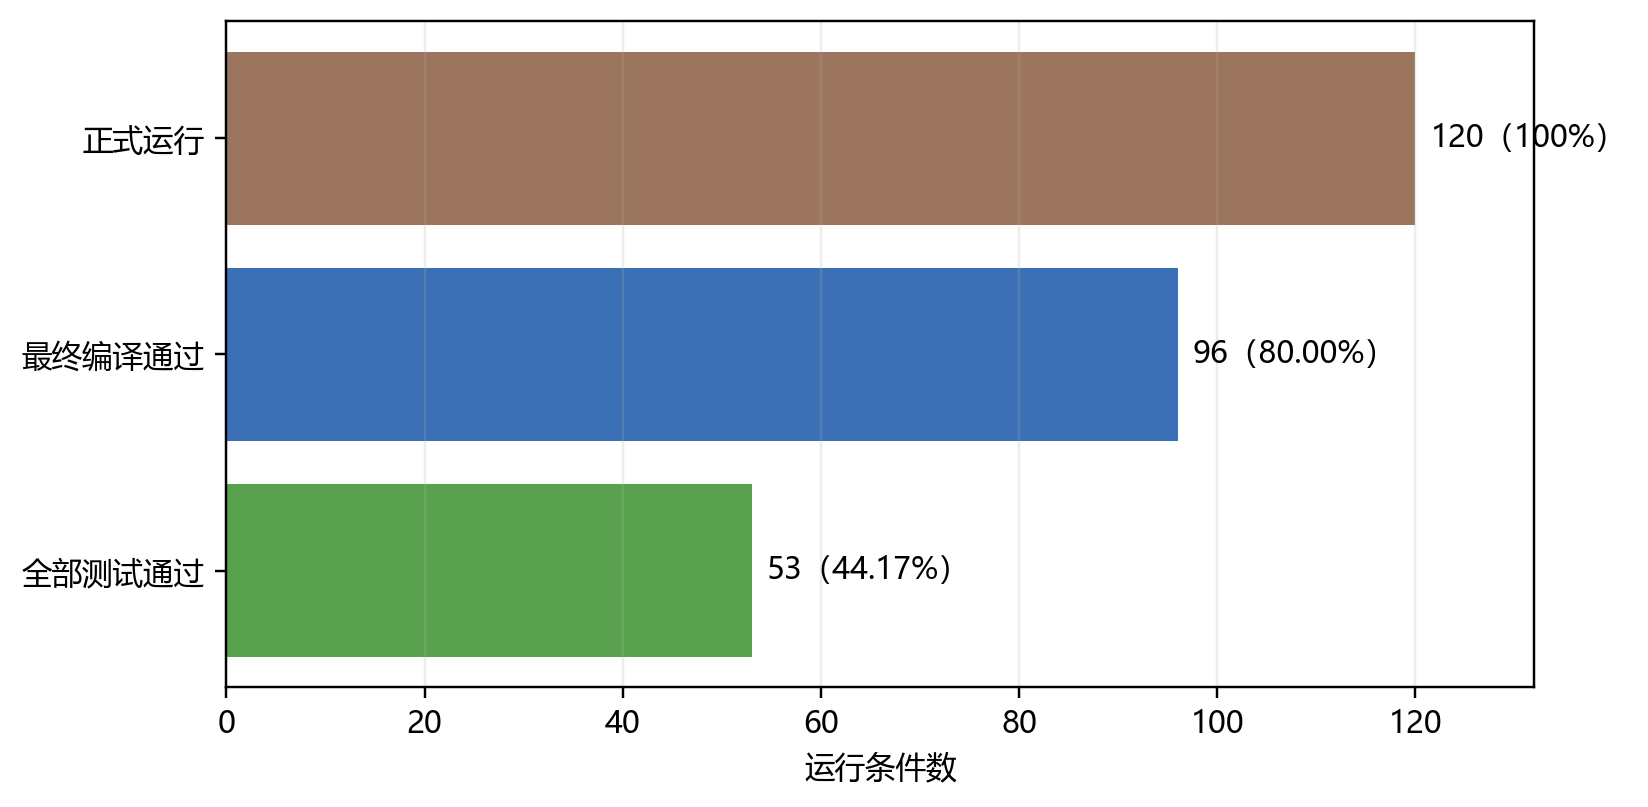
\includegraphics[width=0.78\textwidth]{result_funnel.png}
  \caption{120 次正式运行的结果}
  \label{fig:funnel}
\end{figure}

由图~\ref{fig:funnel} 可得首次编译率为 75.00\%，最终编译率为 80.00\%，测试通过率为 55.71\%，任务成功率为 44.17\%。最终编译率与任务成功率相差 35.83 个百分点，这个差距值得后面分析。

\subsection{四种设置对比}
\begin{table}[H]
  \centering
  \caption{四种设置的正式实验结果}
  \label{tab:four-results}
  \resizebox{\textwidth}{!}{%
  \begin{tabular}{llrrrrrr}
    \toprule
    框架 & 模型 & 首次编译 & 最终编译 & 测试通过 & 任务成功 & 平均修复 & 平均耗时/s\\
    \midrule
    Codex CLI & DeepSeek & 96.67\% & 100.00\% & 77.17\% & 63.33\% & 0.033 & 129.37\\
    Codex CLI & Qwen & 50.00\% & 56.67\% & 39.13\% & 30.00\% & 0.967 & 129.43\\
    自研 harness & DeepSeek & 93.33\% & 100.00\% & 69.57\% & 53.33\% & 0.067 & 119.52\\
    自研 harness & Qwen & 60.00\% & 63.33\% & 36.96\% & 30.00\% & 0.767 & 80.02\\
    \bottomrule
  \end{tabular}}
\end{table}

\begin{figure}[H]
  \centering
  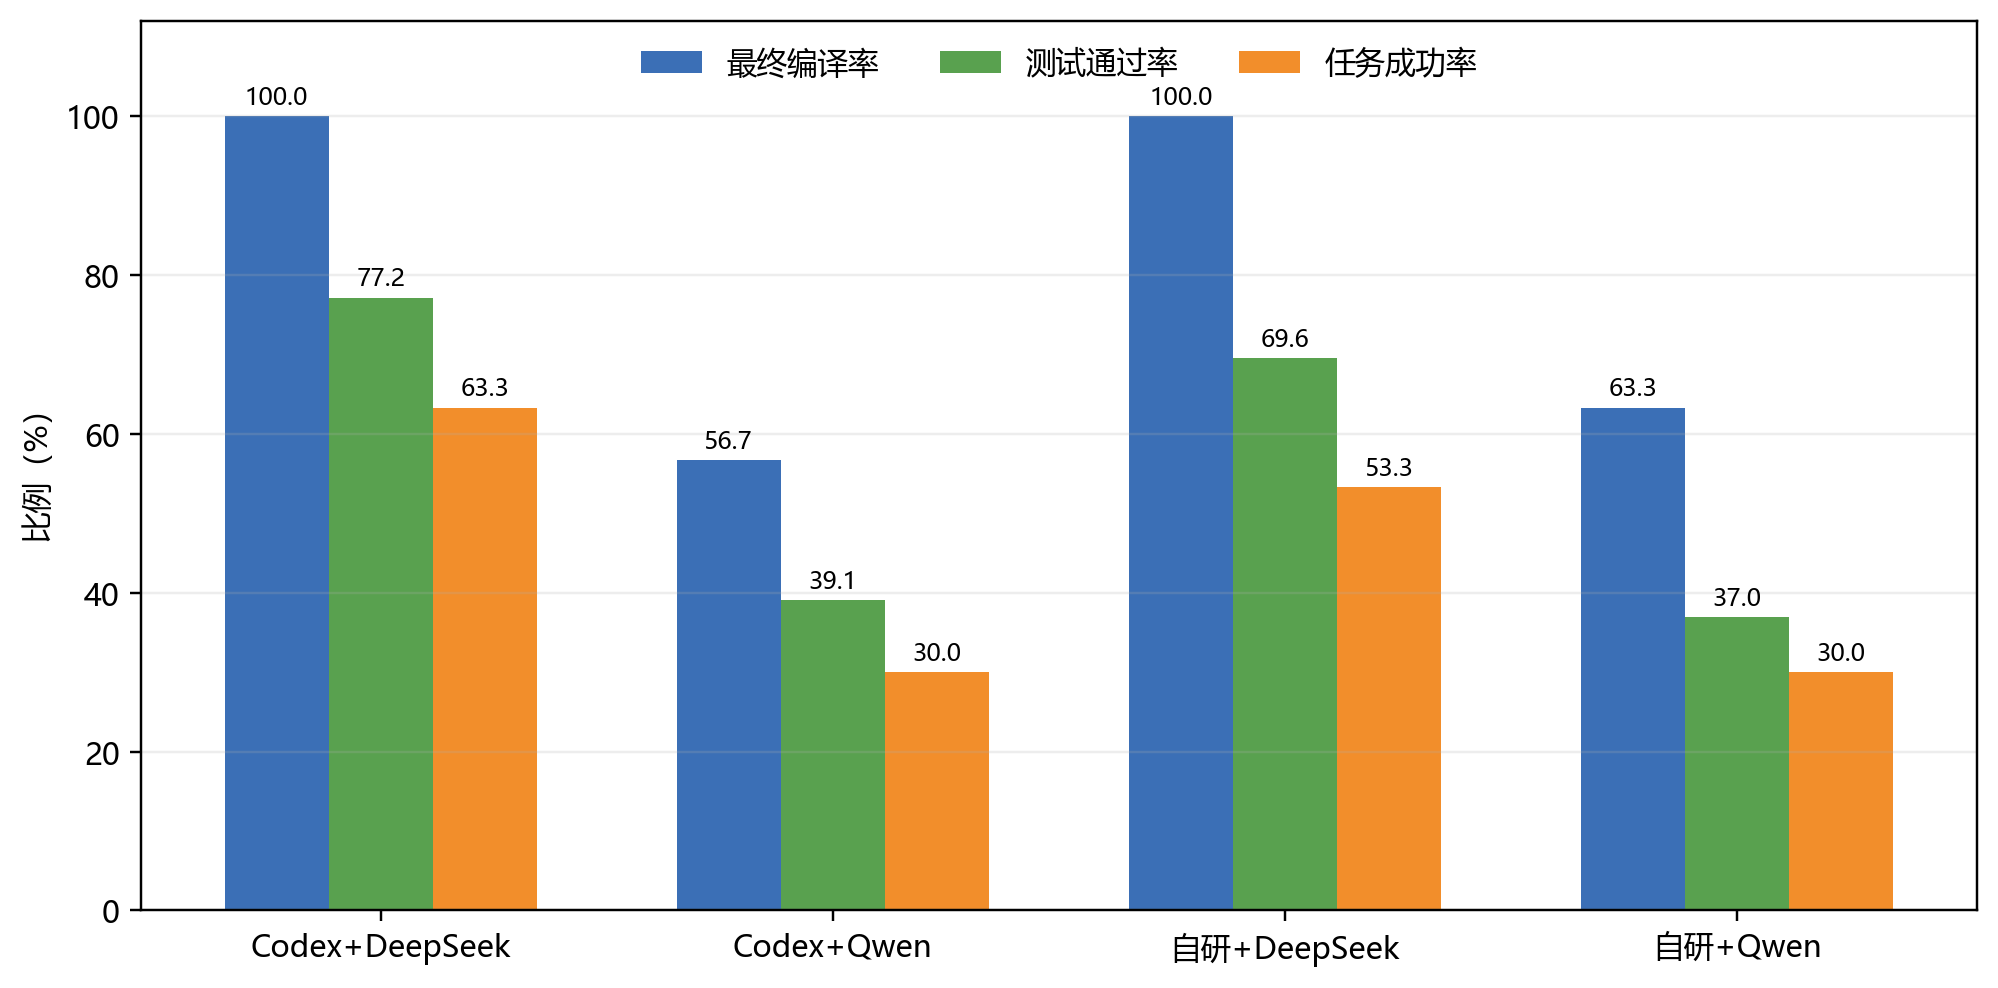
\includegraphics[width=0.98\textwidth]{final_metrics.png}
  \caption{四种设置的最终编译率、测试通过率与任务成功率}
  \label{fig:four-metrics}
\end{figure}

从上面的结果可以看到，Codex CLI + DeepSeek 的三项核心指标最高，不愧是国产模型之光和现在最常用的agent架构呀!它们的任务成功率为 63.33\%；自研 harness + DeepSeek 的任务成功率为 53.33\%。两个 Qwen 设置的任务成功率均为 30.00\%，但自研 harness + Qwen 的最终编译率略高，平均耗时较低。

出于api费用等考虑，我们没有继续搜索比deepseek效果高得多的模型，在最后比较合适的价位找到的qwen，它的效果会差一点，但是也可以作为一个对比，能够发现不是很优秀的模型在我们的项目架构改进的过程中，会发生什么变化。

\subsection{模型框架结果分析}
合并框架数据后，DeepSeek 在 60 次运行中成功 35 次，任务成功率为 58.33\%，测试通过率为 73.37\%；Qwen 成功 18 次，任务成功率为 30.00\%，测试通过率为 38.04\%。合并模型后，Codex CLI 成功 28/60，自研 harness 成功 25/60，对应 46.67\% 和 41.67\%。模型之间的差距明显大于框架之间的总体差距。

\begin{table}[H]
  \centering
  \caption{按难度和题库类型汇总的结果}
  \begin{tabular}{lrr}
    \toprule
    分组 & 任务成功率 & 测试通过率\\
    \midrule
    easy & 61.11\% & 61.11\%\\
    medium & 33.33\% & 51.39\%\\
    hard & 41.67\% & 56.03\%\\
    \midrule
    公共题 & 36.25\% & 48.79\%\\
    自建题 & 60.00\% & 70.00\%\\
    \bottomrule
  \end{tabular}
\end{table}

hard 在本次实验中高于 medium，可能这与具体题目组成和需求表达有关。在前有论述，自建题的需求边界、接口和审核记录更统一，阐述更加规范，所以其总体结果高于公共题。

\begin{figure}[H]
  \centering
  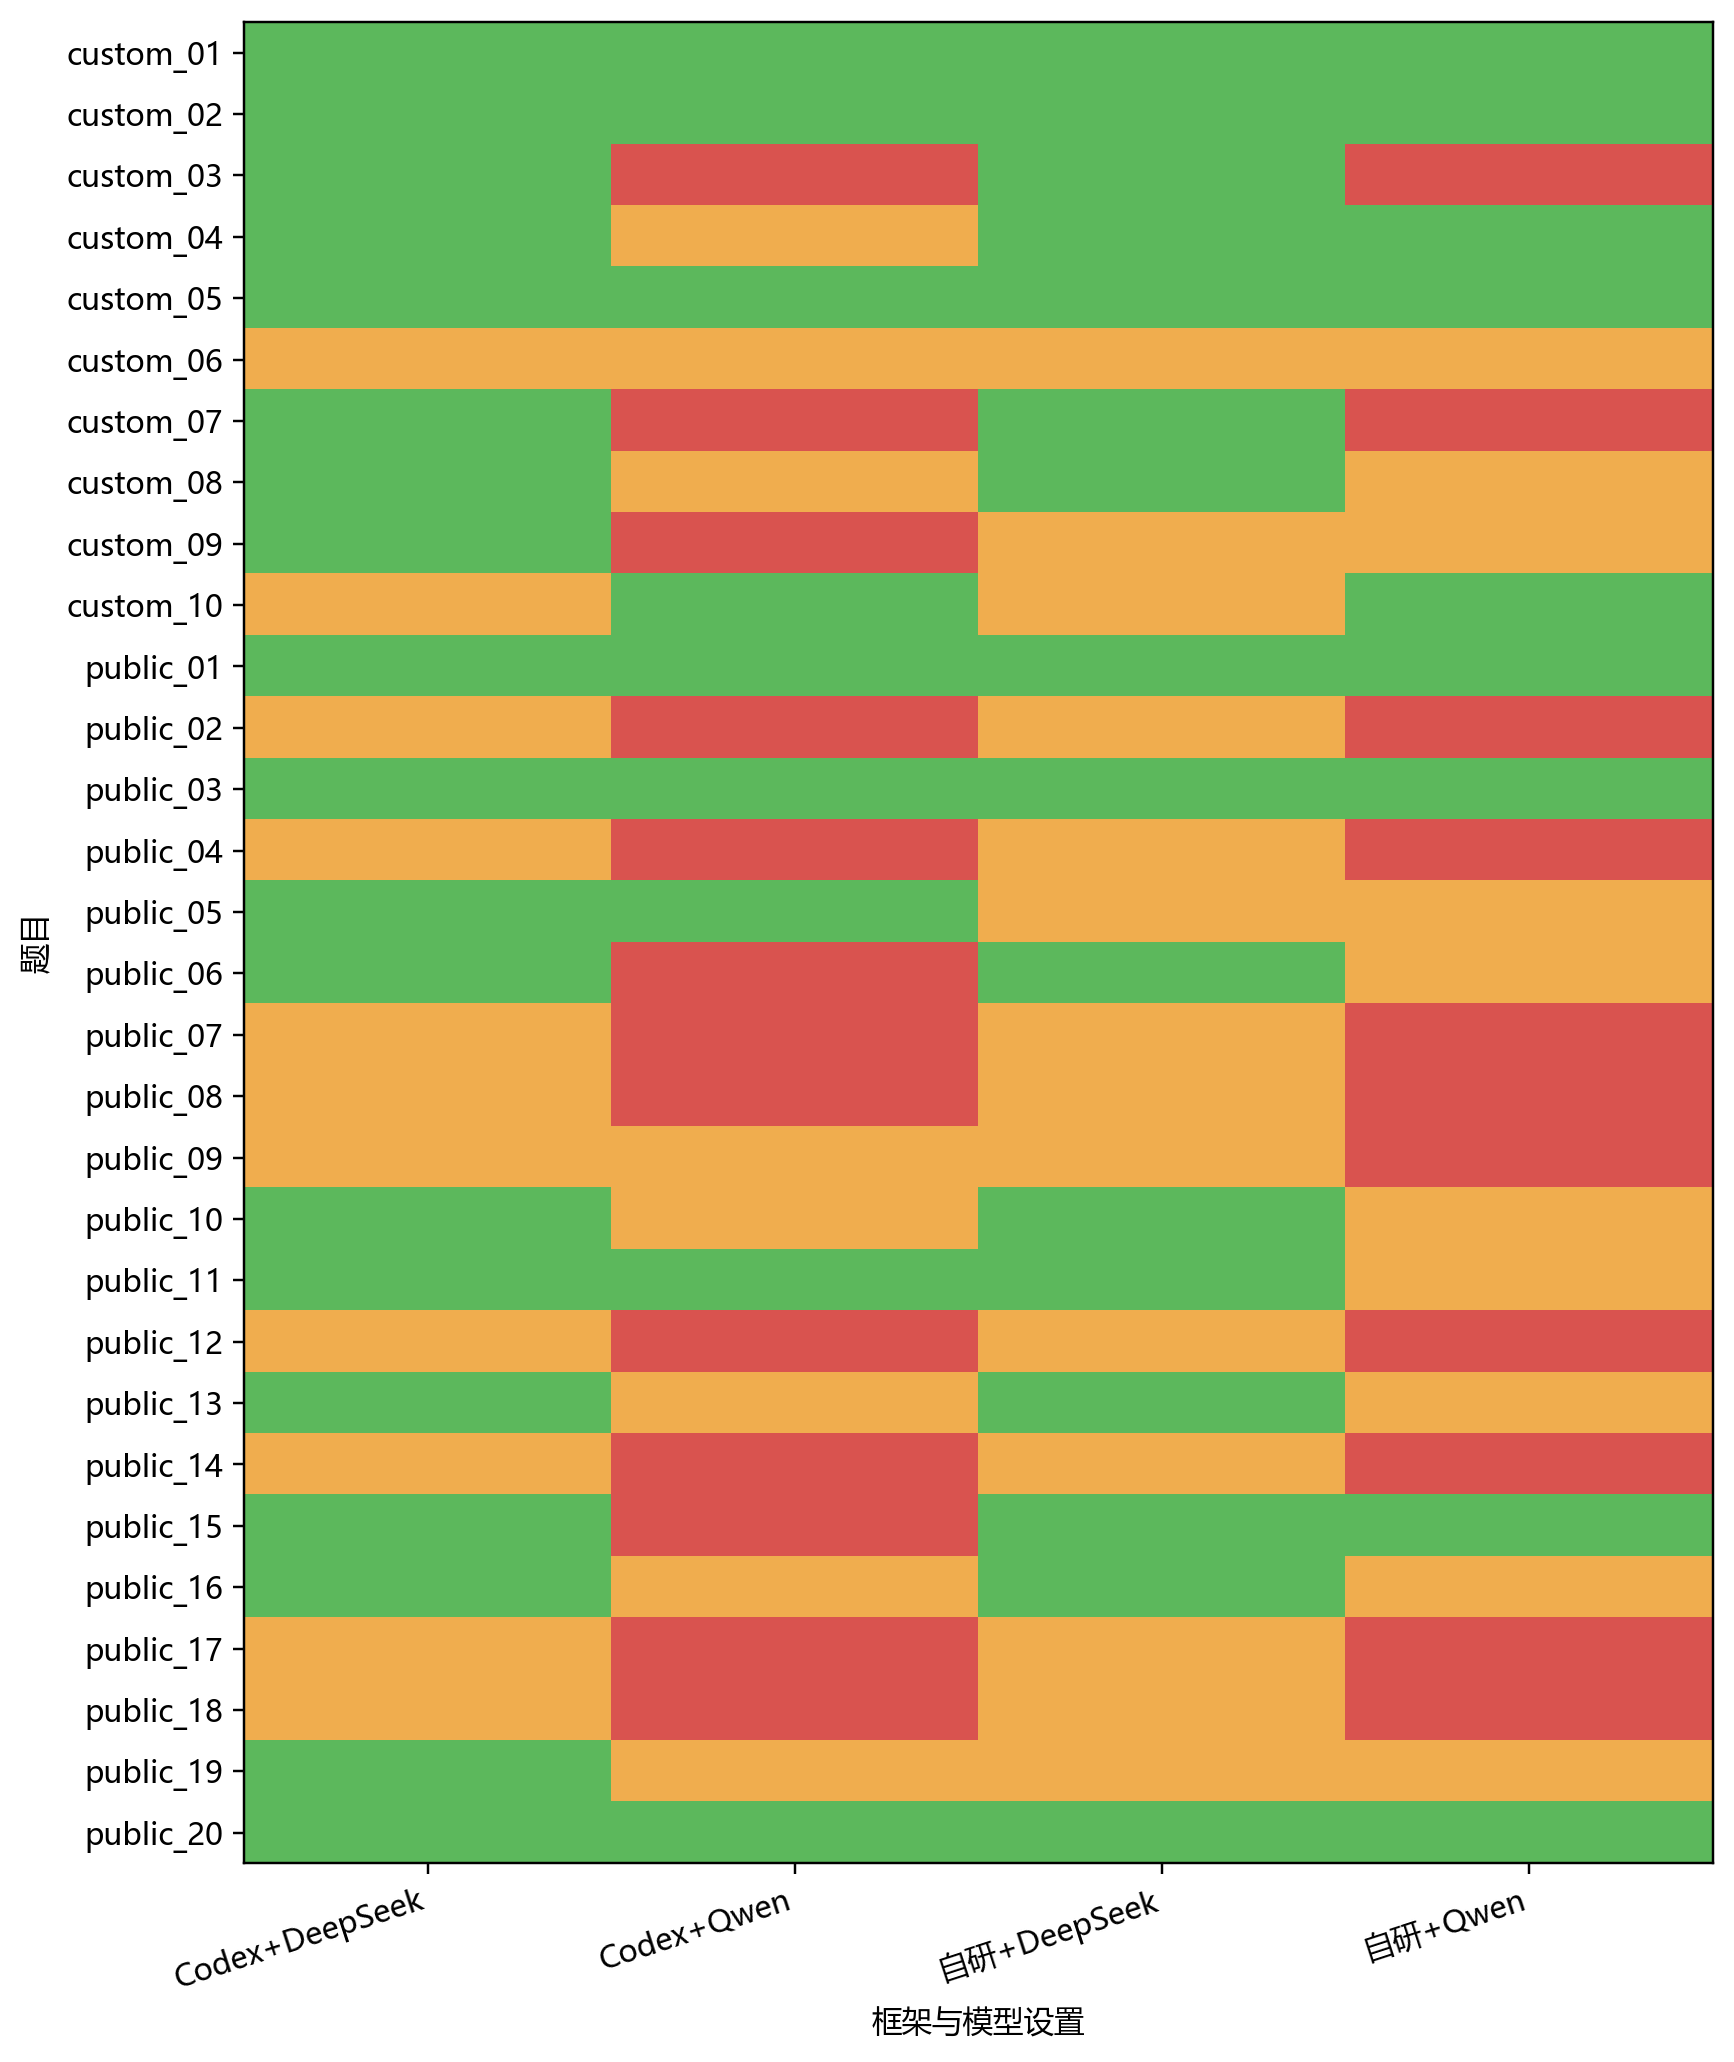
\includegraphics[width=0.83\textwidth]{status_heatmap.png}
  \caption{30 道题在四种设置下的结果（绿：成功；橙：测试失败；红：编译失败）}
  \label{fig:heatmap}
\end{figure}

热力图显示，\texttt{custom\_01}、\texttt{custom\_02}、\texttt{custom\_05}、\texttt{public\_01}、\texttt{public\_03} 和 \texttt{public\_20} 在四组中均成功

\subsection{项目前后改进变化}
为了观察项目改进带来的整体变化，我们比较了两个覆盖相同 120 个条件的完整实验。该比较同时包含上下文、预检和执行方式等系统改进，用于展示迭代结果

\begin{figure}[H]
  \centering
  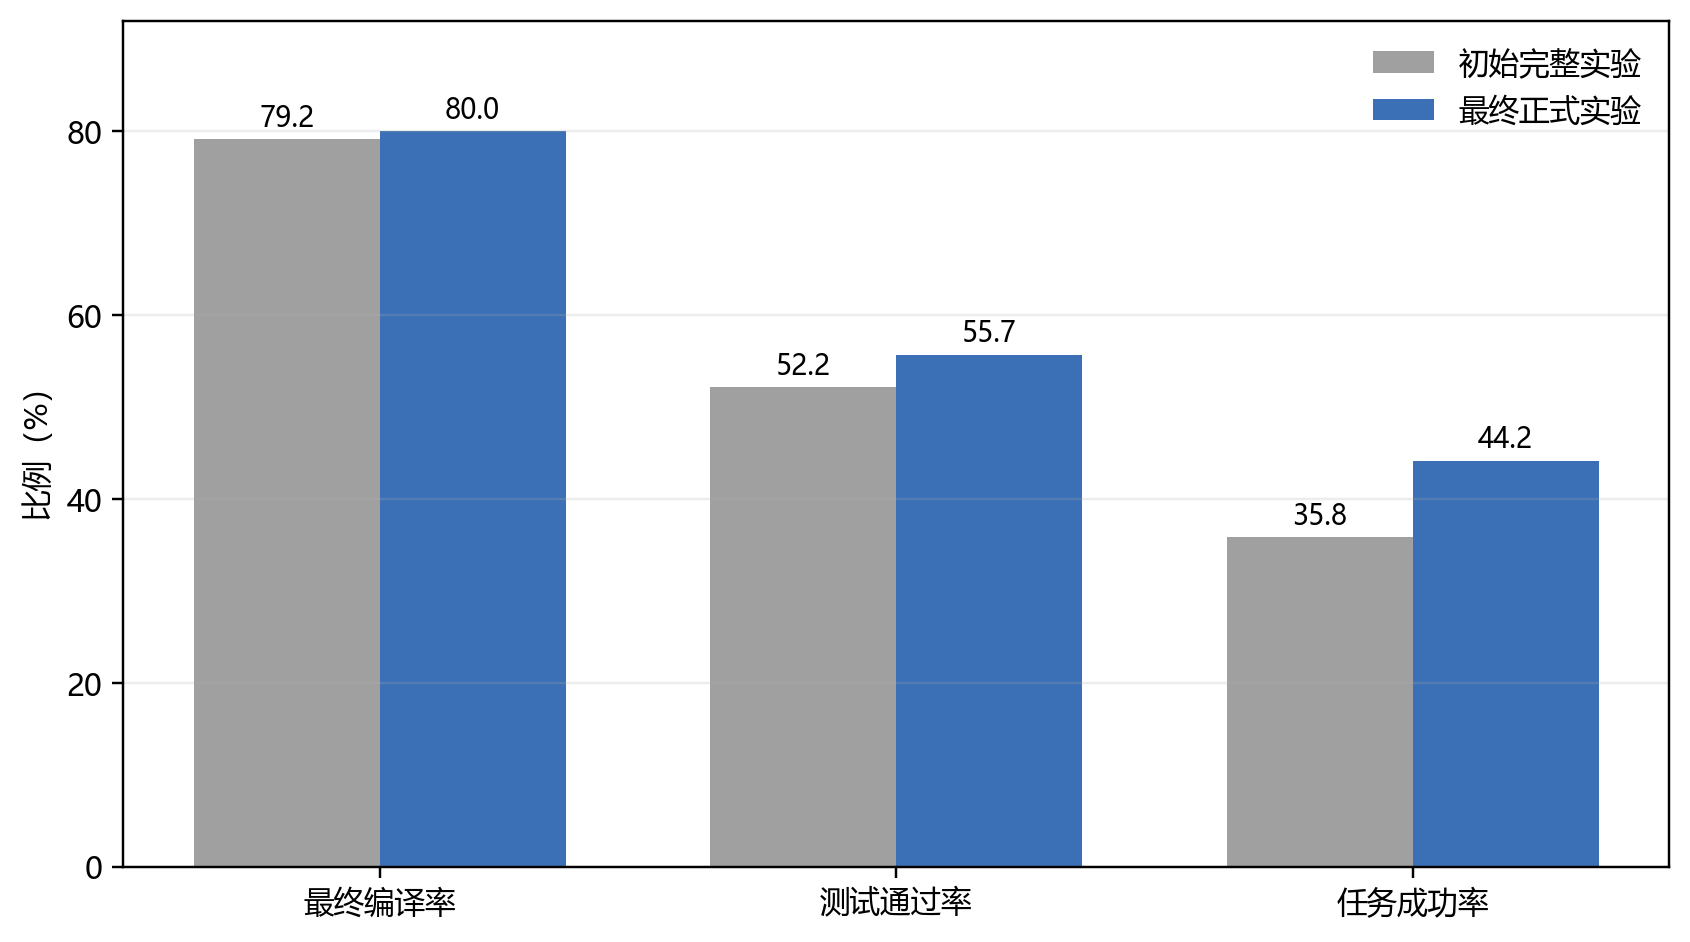
\includegraphics[width=0.78\textwidth]{initial_final_comparison.png}
  \caption{初始完整实验与最终正式实验的核心指标}
  \label{fig:initial-final}
\end{figure}

任务成功数由 43 增加到 53，测试通过数由 192 增加到 205，最终编译数由 95 增加到 96。对应地，任务成功率提高 8.34 个百分点，测试通过率提高 3.54 个百分点。配对比较中有 19 个条件的终态改善，92 个不变，9 个下降。

合并编译与测试后进行查看，原始目录中的 CODESYS 编译/测试进程记录由 271 次减少到 170 次，下降 37.27\%。端到端平均任务耗时由 111.25 s 增至 114.59 s，增加约 3.00\%。外部进程启动减少，但模型响应波动、候选差异和更完整的上下文共同影响了最后执行的时间。因此本次优化主要改善执行结构，但是没有形成稳定的总耗时下降。

\section{结果分析}

\subsection{编译通过与功能分析}
96 个条件通过最终编译，其中 43 个没有通过本题全部测试。这些候选已满足 ST 语法、类型、接口和工程调用链，却在部分需求上不一致。编译器解决的是程序能否进入 PLC 工程，功能测试回答程序在指定场景中做得是否正确，这也是课堂上说的语法和语义的区别。两类证据共同使用，才能判断任务是否完成。

测试通过率 55.71\% 高于任务成功率 44.17\%，也说明不少失败任务并非全部逻辑错误，而是在部分场景中出现偏差。逐步骤记录能够定位第一个不一致的扫描周期，为后续分析提供依据。

\subsection{模型差异}
DeepSeek 在两个框架下均达到 100\% 最终编译率，Qwen 合并后的最终编译率为 60\%。两者的测试通过率分别为 73.37\% 和 38.04\%。从逐题结果看，Qwen 在复杂接口、多模式状态推进和较长上下文下更容易出现编译或功能问题。因此，在本实验的数据集和参数范围内，基座模型能力是影响最终结果的主要因素之一。

害怕额度花完，我们也进行了能够查看范围内的token记录。Token记录也呈现出不同调用特征，Codex CLI + Qwen 的总 Token 为 3,248,894，明显高于其他三组；自研 harness 的两个模型合计 Token 较少。Codex的agent架构可能会引入更多的上下文和更多请求，增加token消耗。

\subsection{框架差异}
Codex CLI 的总体任务成功率为 46.67\%，自研 harness 为 41.67\%，相差 5 个百分点。即使是换用很好的框架，也不能非常大幅提高成功率。DeepSeek 下 Codex CLI 高 10 个百分点，Qwen 下两者任务成功率相同；自研 harness + Qwen 的最终编译率高 6.66 个百分点，框架影响会随模型和题目变化。

自研 harness 的价值还体现在实验控制能力，它能够更加符合我们的需求。任务上下文、候选格式、修复上限、外部工具调用、测试隔离和证据目录都有明确边界，它没有依赖多 Agent 编排或复杂插件系统，主要模块可以直接追踪到课程要求中的生成、编译、修复、测试和公平比较。

下面对几个结果进行分析：

\subsection{成功案例：\texttt{public\_20}}
\texttt{public\_20} 是五工位生产控制任务，难度为 hard，包含多工位状态和协同控制。四种设置均通过编译并通过 4/4 测试。该结果说明，当题目的模式边界、接口和状态推进足够明确时，不同框架和模型都可能形成可执行的完整控制逻辑。

这个案例也解释了 hard 组结果没有低于 medium 的一部分原因，难度标签描述任务包含的结构，但题面表达质量和测试路径同样影响模型表现。\texttt{public\_20} 虽然状态较多，流程关系相对清晰。

\subsection{语义失败案例：\texttt{custom\_06}}
\texttt{custom\_06} 描述填充、混合、排空三个阶段。四种设置全部通过编译，但没有一组通过全部测试；四组共通过 6/12 个测试。候选能够建立基本状态机，却会在阶段退出、计时完成或复位后的状态上产生偏差。

这个案例说明了编译通过不等于功能正确。若实验只记录编译结果，四组都会被判为成功；加入共享测试后，才能发现多阶段任务中的控制语义问题。

\subsection{组合差异案例：\texttt{public\_19}}
\texttt{public\_19} 包含手动、单步、单周期和连续模式。四种设置都通过编译，只有 Codex CLI + DeepSeek 通过全部 4 个测试，其余三组存在功能失败。该题需要同时处理模式互斥、状态推进和复位，模型与框架组合会影响上下文理解和最终控制结构。

\subsection{失败类型与局限}

由于时间限制，本实验仍有部分局限。第一，正式结果来自一台计算机和一个 CODESYS 版本。第二，每个条件正式运行一次，无法估计模型输出方差。第三，初始到最终实现同时修改多个部分，完整实验对比不能分离单项贡献。第四，LTL 用于需求组织和上下文，尚未接入 PLCVerif。第五，92 个测试只能覆盖主要行为，仍不能穷尽所有输入和状态。

\section{结论}
本项目围绕 PLC ST 代码生成建立了完整、可执行的实验链路。数据部分包含 30 道题、136 条 LTL 性质、92 个测试用例和 352 个测试步骤；系统部分实现了自研 harness、Codex CLI 基线、两个模型接入、CODESYS 编译和 Simulation 自动测试；实验部分完成了四种设置共 120 次正式运行，并保存从原始响应到逐步骤测试结果的证据。


项目改进围绕真实问题逐步展开。本地预检能够减少无效外部调用，LTL 上下文补充语义约束，编译与测试合并减少重复 CODESYS 启动。

最终实验的首次编译率为 75.00\%，最终编译率为 80.00\%，测试通过率为 55.71\%，任务成功率为 44.17\%。DeepSeek 的总体表现明显高于 Qwen，两个框架的总体差距相对较小。96 个可编译条件中有 43 个仍存在功能失败，说明 PLC 代码生成的主要难点已经从语法完整延伸到状态、优先级和时序语义。


\appendix
\section{电子附录与证据目录}
完整题目位于 \path{data/tasks/}，逐题 LTL 位于 \path{data/specs/}，共享测试位于 \path{data/test_cases/}。最终正式实验原始证据位于 \path{experiments/raw/formal/20261111_102220_v4_formal/}；报告使用的逐任务汇总、四组汇总和初始—最终对比分别保存在 \path{experiments/processed/} 下。本文中的表格和图片由 \path{experiments/analysis/} 中的脚本从上述 JSON 生成。

\section{报告数字追溯表}
\begin{longtable}{L{4.0cm}L{5.3cm}L{4.0cm}}
  \toprule
  报告内容 & 处理后数据 & 原始来源\\
  \midrule
  \endfirsthead
  \toprule
  报告内容 & 处理后数据 & 原始来源\\
  \midrule
  \endhead
  四种设置结果 & \path{formal_summary.json/csv} & 最终正式批次 120 个运行目录\\
  逐题终态与耗时 & \path{formal_runs.json/csv} & 每个条件的 \path{run_result.json}\\
  初始与最终对比 & \path{initial_final_comparison.json/csv} & 两个完整正式批次\\
  报告分析表 & \path{formal_analysis.md} & 汇总脚本自动生成\\
  图~\ref{fig:four-metrics}、\ref{fig:heatmap}、\ref{fig:initial-final} & \path{generate_report_figures.py} & 处理后 JSON\\
  \bottomrule
\end{longtable}

\end{document}
